\documentclass[tikz,border=10pt]{standalone}
\usepackage{tikz}
\usetikzlibrary{arrows.meta}

% ---------- Color palette ----------
\definecolor{idtoken}{RGB}{37,99,235}      % blue    - ID Token
\definecolor{acctoken}{RGB}{21,128,61}     % green   - Access Token
\definecolor{svctoken}{RGB}{194,65,12}     % orange  - Service Token
\definecolor{ctrlgray}{RGB}{75,85,99}      % gray    - trust verification / control plane

\definecolor{userzoneline}{RGB}{185,28,28}
\definecolor{userzonefill}{RGB}{254,242,242}
\definecolor{idzoneline}{RGB}{29,78,216}
\definecolor{idzonefill}{RGB}{239,246,255}
\definecolor{ztzoneline}{RGB}{15,118,110}
\definecolor{ztzonefill}{RGB}{240,253,250}

\begin{document}
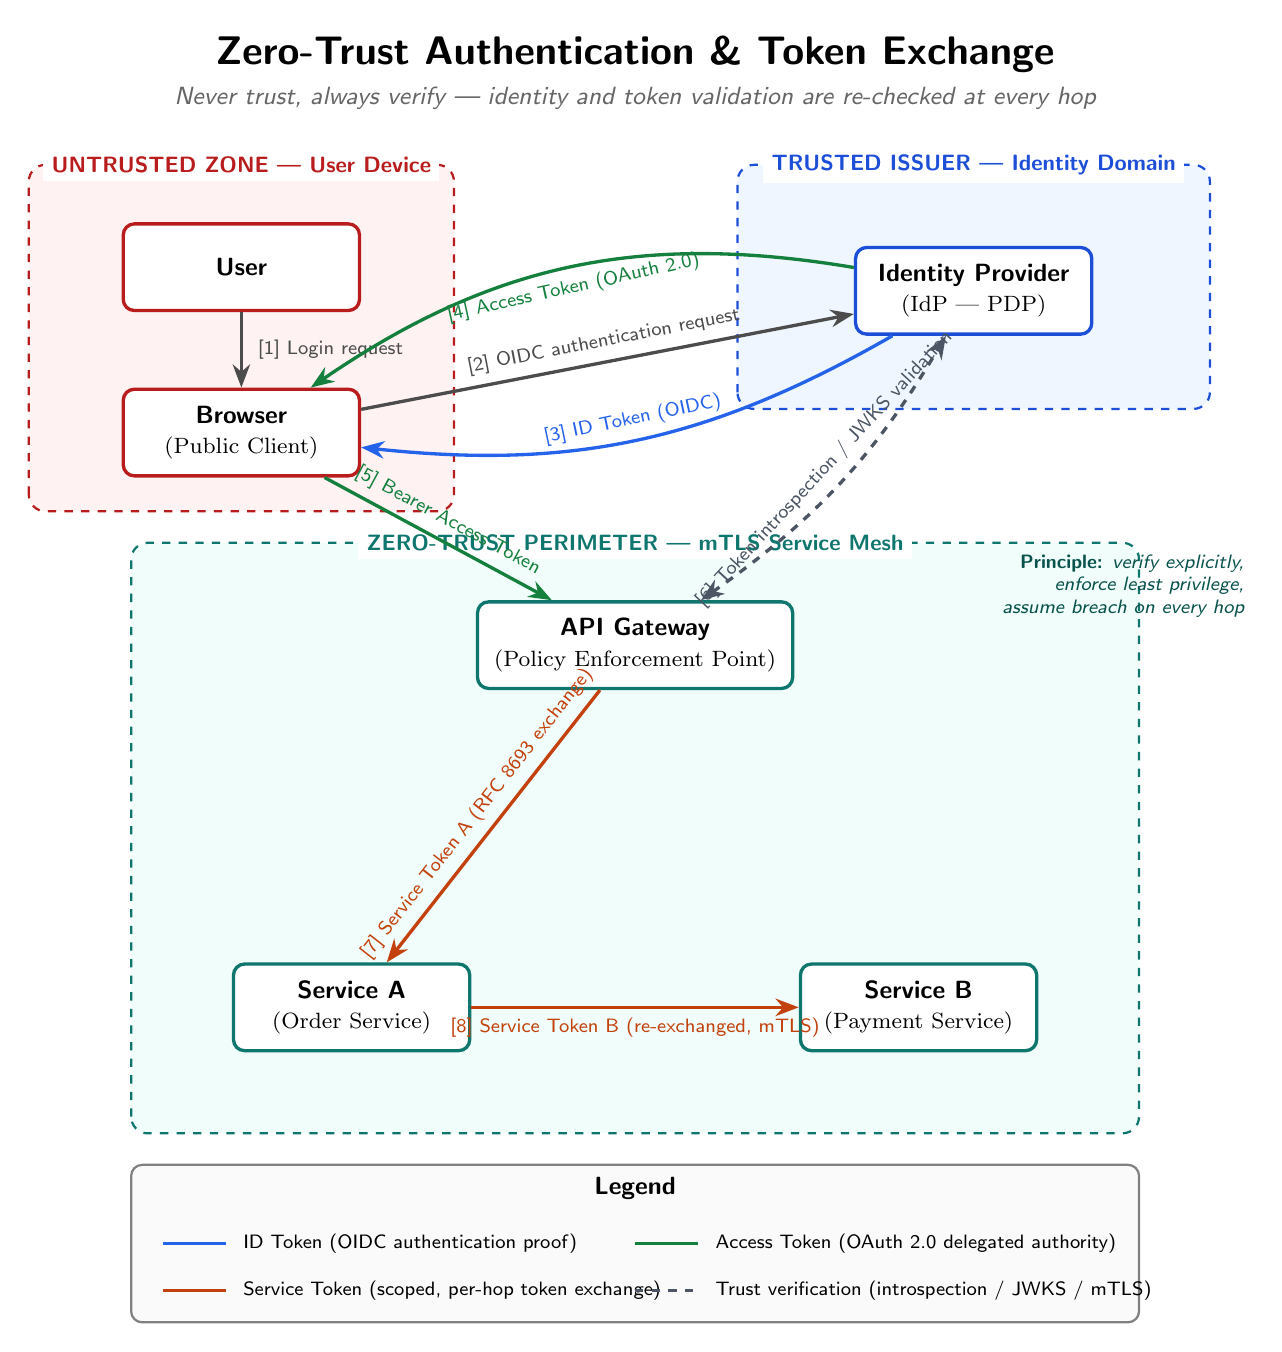
\begin{tikzpicture}[
  >=Stealth,
  font=\sffamily,
  actor/.style={
    rectangle, rounded corners=4pt, very thick,
    fill=white, minimum width=3.0cm, minimum height=1.1cm,
    align=center, font=\sffamily\bfseries\small, inner sep=6pt
  },
  zonelabel/.style={
    font=\sffamily\bfseries\footnotesize, fill=white, inner sep=3pt, draw=none
  },
  flowlabel/.style={font=\sffamily\scriptsize, align=center}
]

% =====================================================================
% Title
% =====================================================================
\node[font=\sffamily\bfseries\Large] at (8.0,14.1) {Zero-Trust Authentication \& Token Exchange};
\node[font=\sffamily\itshape\small, text=black!60] at (8.0,13.55)
  {Never trust, always verify --- identity and token validation are re-checked at every hop};

% =====================================================================
% Trust boundary regions
% =====================================================================

% -- User Domain (untrusted public zone) --
\draw[userzoneline, thick, dashed, rounded corners=6pt, fill=userzonefill]
  (0.3,8.3) rectangle (5.7,12.7);
\node[zonelabel, text=userzoneline] at (3.0,12.7)
  {UNTRUSTED ZONE --- User Device};

% -- Identity Provider Domain (trusted issuer) --
\draw[idzoneline, thick, dashed, rounded corners=6pt, fill=idzonefill]
  (9.3,9.6) rectangle (15.3,12.7);
\node[zonelabel, text=idzoneline] at (12.3,12.7)
  {TRUSTED ISSUER --- Identity Domain};

% -- Zero-Trust Perimeter (mTLS service mesh) --
\draw[ztzoneline, thick, dashed, rounded corners=6pt, fill=ztzonefill]
  (1.6,0.4) rectangle (14.4,7.9);
\node[zonelabel, text=ztzoneline] at (8.0,7.9)
  {ZERO-TRUST PERIMETER --- mTLS Service Mesh};
\node[font=\sffamily\itshape\scriptsize, text=ztzoneline!70!black, align=right]
  at (14.2,7.35) {\textbf{Principle:} verify explicitly,\\ enforce least privilege,\\ assume breach on every hop};

% =====================================================================
% Actors
% =====================================================================
\node[actor, draw=userzoneline] (User) at (3.0,11.4) {User};
\node[actor, draw=userzoneline] (Browser) at (3.0,9.3)
  {Browser\\{\footnotesize\normalfont (Public Client)}};

\node[actor, draw=idzoneline] (IdP) at (12.3,11.1)
  {Identity Provider\\{\footnotesize\normalfont (IdP --- PDP)}};

\node[actor, draw=ztzoneline] (Gateway) at (8.0,6.6)
  {API Gateway\\{\footnotesize\normalfont (Policy Enforcement Point)}};
\node[actor, draw=ztzoneline] (ServiceA) at (4.4,2.0)
  {Service A\\{\footnotesize\normalfont (Order Service)}};
\node[actor, draw=ztzoneline] (ServiceB) at (11.6,2.0)
  {Service B\\{\footnotesize\normalfont (Payment Service)}};

% =====================================================================
% Flows
% =====================================================================

% [1] User -> Browser
\draw[->, very thick, black!70] (User) -- (Browser)
  node[flowlabel, midway, right, xshift=2pt] {[1] Login request};

% [2] Browser -> IdP : authentication request
\draw[->, very thick, black!70] (Browser) -- (IdP)
  node[flowlabel, midway, above, sloped] {[2] OIDC authentication request};

% [3] IdP -> Browser : ID Token
\draw[->, very thick, idtoken] (IdP) to[bend left=18]
  node[flowlabel, midway, above, sloped, text=idtoken] {[3] ID Token (OIDC)}
  (Browser);

% [4] IdP -> Browser : Access Token
\draw[->, very thick, acctoken] (IdP) to[bend right=22]
  node[flowlabel, midway, below, sloped, text=acctoken] {[4] Access Token (OAuth 2.0)}
  (Browser);

% [5] Browser -> Gateway : bearer access token presented at the perimeter
\draw[->, very thick, acctoken] (Browser) -- (Gateway)
  node[flowlabel, midway, above, sloped, text=acctoken] {[5] Bearer Access Token};

% [6] Gateway <-> IdP : token introspection / JWKS validation
\draw[<->, very thick, dashed, ctrlgray] (Gateway) to[bend right=12]
  node[flowlabel, midway, above, sloped, text=ctrlgray] {[6] Token introspection / JWKS validation}
  (IdP);

% [7] Gateway -> Service A : scoped-down service token (RFC 8693 exchange)
\draw[->, very thick, svctoken] (Gateway) -- (ServiceA)
  node[flowlabel, midway, above, sloped, text=svctoken] {[7] Service Token A (RFC 8693 exchange)};

% [8] Service A -> Service B : re-minted, further-scoped service token over mTLS
\draw[->, very thick, svctoken] (ServiceA) -- (ServiceB)
  node[flowlabel, midway, below, text=svctoken] {[8] Service Token B (re-exchanged, mTLS)};

% =====================================================================
% Legend
% =====================================================================
\draw[black!50, thick, rounded corners=4pt, fill=black!2]
  (1.6,-2.0) rectangle (14.4,0.0);
\node[font=\sffamily\bfseries\small] at (8.0,-0.3) {Legend};

\draw[idtoken, very thick] (2.0,-1.0) -- (2.8,-1.0);
\node[flowlabel, anchor=west] at (2.9,-1.0) {ID Token (OIDC authentication proof)};

\draw[acctoken, very thick] (8.0,-1.0) -- (8.8,-1.0);
\node[flowlabel, anchor=west] at (8.9,-1.0) {Access Token (OAuth 2.0 delegated authority)};

\draw[svctoken, very thick] (2.0,-1.6) -- (2.8,-1.6);
\node[flowlabel, anchor=west] at (2.9,-1.6) {Service Token (scoped, per-hop token exchange)};

\draw[ctrlgray, very thick, dashed] (8.0,-1.6) -- (8.8,-1.6);
\node[flowlabel, anchor=west] at (8.9,-1.6) {Trust verification (introspection / JWKS / mTLS)};

\end{tikzpicture}
\end{document}
